\documentclass[12pt,a4paper]{article}
\usepackage[utf8]{inputenc}
\usepackage[german]{babel}
\usepackage[T1]{fontenc}
\usepackage{amsmath}
\usepackage{amsfonts}
\usepackage{amssymb}
\usepackage{graphicx}
\usepackage[left=2.5cm,right=2.5cm,top=2cm,bottom=2cm]{geometry}
\usepackage{float}
\usepackage{subfigure}
\author{Gruppe C14 \\ Julián Häck, Martin Koytek, Lars Wenning, Erik Zimmermann}
\begin{document}
\section{Gedämpfter LC Schwingkreis Oszilloskop, Teilversuch 4.4.1}
\subsection{Versuchsbeschreibung}
Kurze Darstellung der physikalischen Grundlagen und Ziele der Versuche, die zum Verständnis
des Versuches/Protokolls benötigt werden. (max. 1 Seite)
Messung der Frequenz f und des Abklingkoeffizienten $\delta$ eines LC-Schwingkreises mit dem Oszilloskop.
\begin{equation}
U=U_0\cdot e^{- \frac{t}{\tau}}
\end{equation}

\subsection{Versuchsaufbau und Durchführung}
Genaue Beschreibung der verwendeten Aufbauten unter Verwendung von Skizzen oder Photos
Beschreibung der Messwerterfassungseinstellungen (eingestellte Messzeiten, Messbedingungen,
Trigger, Anzahl der Messungen) und der Durchführung der Versuche. (max. 1 Seite)\newline

\begin{figure}[H]
\centering
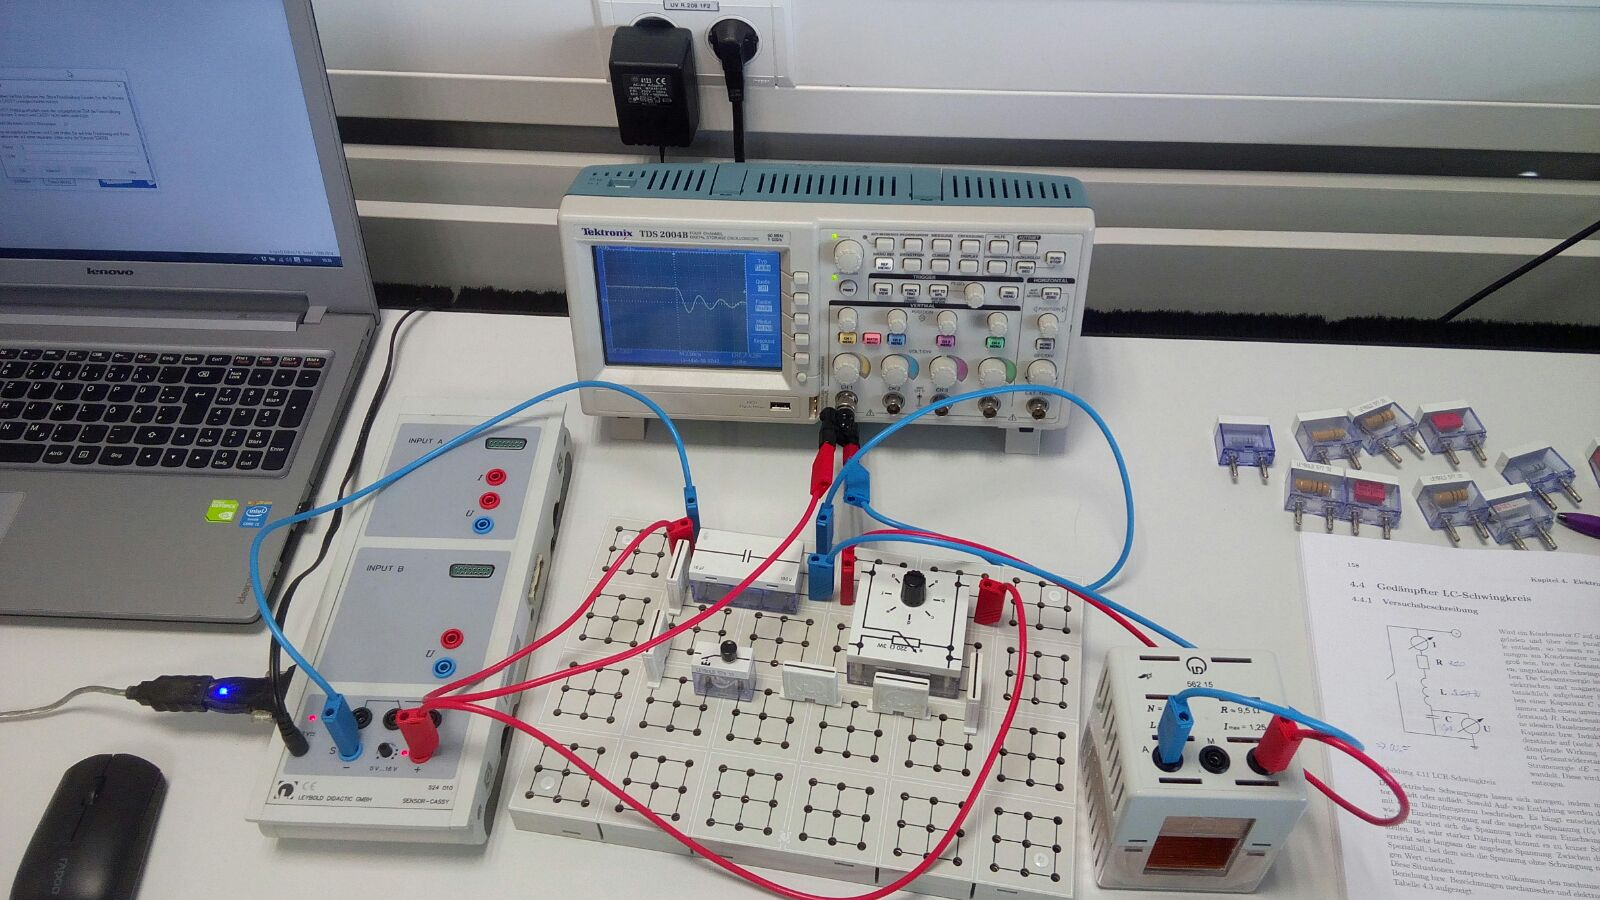
\includegraphics[scale=0.27]{ArbeitsplatzE_1.jpg}
\caption{Versuchsaufbau}
\end{figure}


\begin{itemize}
\item Bei dem oben gezeigten LRC Schwingkreis wurde der Drehwiderstand komplett herunter geregelt ($R=0.02\Omega$). Dieser wird erst später in Versuch 4.4.2 gebraucht. Bei dem verbleibenden gedämpften LC-Schwingkreis wird die Spannung über dem Kondensator mit dem Oszilloskop aufgezeichnet, um die Frequenz und den Abklingkoeffizienten zu bestimmen.  
\item Alle Versuche wurden bei einer Eingangspannung von $U_0=5.6V$ durchgeführt, dabei wurde das Oszilloskop auf \glqq Single Sequence\grqq eingestellt und aus dem resultierenden Standbild die Spannungsmaxima mit entsprechenden Zeitwerten abgelesen. Dazu wurden die Messbereiche auf $U_B=16V$ (Spannung) \& $T_B=50*10^{-3}s$ (Zeit) eingestellt.
\item Es lag ein Offset von $off=50*10^{-3}V$ vor, der im Folgenden ausgeglichen wurde.
\item Die Ablesefehler wurden zu $\sigma_U=\frac{0.08}{\sqrt{12}}V$ \& $\sigma_T=\frac{100*10^{-6}}{\sqrt{12}}s$ bestimmt.
Diese Messung wurde 4 mal wiederholt wobei die Ergebnisse des 2. Versuchs aufgrund eines Stromausfalls verloren gingen.
\end{itemize}

\newpage
\subsection{Versuchsauswertung}

\subsubsection{Rohdaten}
\begin{itemize}

\item Spule (Herstellerangaben):\centering
\end{itemize}
\begin{figure}[H]\centering
\begin{tabular}{c|l}
Induktivität & $L=36*10^{-3}H$\\ 
Windungen & $N=1000$\\ 
Widerstand & $R=9.5\Omega$ \\
\end{tabular} 
\end{figure}

\begin{itemize}
\item Kondensator (Herstellerangabe):\centering
\end{itemize}
\begin{figure}[H]\centering
\begin{tabular}{c|l}
Kapazität & $C=10*10^{-6}F$\\ 
\end{tabular} 
\end{figure}

\begin{itemize}
\item Messdaten\centering
\end{itemize}
\begin{table}[H]\centering
\caption{1. Messung}
\begin{tabular}{c|c}
$U_1=3.12V$& $t_1=0.5ms$\\ 
$U_2=1.76V$& $t_2=4.4ms$\\ 
$U_3=1.04V$& $t_3=8.2ms$ \\
$U_4=0.56V$& $t_4=12.0ms$ \\
\end{tabular} 
\end{table}

2. Messung fehlt wegen Stromausfall. \centering

\begin{table}[H]\centering
\caption{3. Messung}
\begin{tabular}{c|c}
$U_1=3.2V$& $t_1=0.5ms$\\ 
$U_2=1.76V$& $t_2=4.4ms$\\ 
$U_3=1.04V$& $t_3=8.2ms$ \\
$U_4=0.64V$& $t_4=12.0ms$ \\
$U_5=0.4V$& $t_4=15.9ms$ \\
\end{tabular} 
\end{table}

\begin{table}[H]\centering
\caption{4. Messung}
\begin{tabular}{c|c}
$U_1=3.12V$& $t_1=0.5ms$\\ 
$U_2=1.76V$& $t_2=4.4ms$\\ 
$U_3=1.12V$& $t_3=8.2ms$ \\
$U_4=0.8V$& $t_4=12.1ms$ \\
$U_5=0.4V$& $t_4=15.9ms$ \\
\end{tabular} 
\end{table}
$U_4$ und $T_4$ wurden bei Messung4 wegen falschem Ablesen verworfen.

\newpage
\subsubsection{Transformation der Rohdaten}
Transformation der Rohdaten und Modellanpassung. (1 Seite)\\
Die Frequenzen wurden aus den Differenzen der Zeitabstände $T_i$ bestimmt. Bestimmung von Delta siehe (\ref{Peter}) \\
Beispiel:

\begin{table}[H]\centering
\caption{Messung 1}
\begin{tabular}{c|c|c|c}
Frequenz in Hz & $\sigma_f$ in Hz & Abklingkoeffizient in $\frac{1}{s}$ & $\sigma_{\delta}$ in $\frac{1}{s}$\\ 
\hline
$f=256.410$& $\sigma_f=1.898$& $\delta=150.047$& $\sigma_{\delta}=4.264$\\ 
$f=263.158$& $\sigma_f=1.999$& $\delta=143.827$& $\sigma_{\delta}=7.260$\\
$f=263.158$& $\sigma_f=1.999$& $\delta=174.551$& $\sigma_{\delta}=13.535$\\
\end{tabular} 
\end{table}
Hier wurden die Fehler aus den folgenden Gleichungen ermittelt:
\begin{align}
\sigma_f&=\frac{\sigma_T}{T^2}\\
\sigma_{\delta_n}=\frac{1}{T_n}\cdot \sqrt{(\frac{\sigma_{U_n}}{U_n})^2+(\frac{\sigma_{U_{n+1}}}{U_{n+1}})^2+(\delta_n\cdot \sigma{T_n})^2}
\end{align}
Der Abklingkoeffizient $\delta$ wird bestimmt aus:

\begin{align}
U_{n+1}&=U_n \cdot e^{-\delta \cdot (t_{n+1}-t_n)}\notag \\
\Rightarrow \hspace{0.5cm} \delta_n&=\frac{\ln{\frac{U_n}{U_{n+1}}}}{t_{n+1}-t_n}
\label{Peter}
\end{align}
\newline
Aus den Einzelmessungen haben wir für die Frequenz und den Abklingkoeffizient den gewichteten Mittelwert mit seinem Fehler bestimmt:

\begin{table}[H]\centering
\caption{Messung 1}
\begin{tabular}{c|c|c|c}
gemittelte Frequenz in Hz& $\sigma_{\bar{f}}$ in Hz & gemittelter Abklingkoeffizient in $\frac{1}{s}$ & $\sigma_{\bar{\delta}}$ in $\frac{1}{s}$\\ 
\hline
$\bar{f}=259.960$&$\bar{\sigma_f}= 0.617$& $\bar{\delta}=148.025$& $\sigma_{\bar{\delta}}=1.994$\\ 
\end{tabular} 
\end{table}
\newpage
\subsubsection{Analyse}
Analyse der Daten inklusive Fehlerrechnung Residuen und Pullverteilung. (1 Seite)
\subsubsection{Fazit}
Diskussion der Ergebnisse und Vergleich der erzielten Ergebnisse mit theoretischen Vorhersagen.
(1 Seite)

\end{document}